\documentclass{mobileappdev}
\usepackage[utf8]{inputenc}
\usepackage[ngerman]{babel}
\usepackage{ amssymb }

\begin{document}

\maketitle{}{Prof. Dr. Johannes Schöning}{}

\underline{\textbf{App Name:}} Sannad

Wir haben uns für den Namen Sannad entschieden, weil dieser übersetzt aus dem Arabischen ''Hilfe'' bedeutet. Der Grund dazu ist, dass unsere App Menschen die Möglichkeit geben soll, sich gegenseitig zu helfen.

\underline{\textbf{Plattform:}} Android

 \underline{\textbf{Grobe Idee:}} Jeder soll die Möglichkeit bekommen, durch einen Tap auf seinem Handy hilfe zu bekommen. Dieses gilt vor allem für alte Leute, und Leute die in Quarantäne sitzen, und nicht alleine Einkaufen gehen können bzw. dürfen und ähnliches.

Wir möchten diese App aber auch nach der Korona-Kriese weiterbenutzen, und ermöglichen deswegen den Benutzern um alle Arten von Hilfe zu bitten bzw. anzubieten. Dieses könnte alles mögliche von Einkaufen zu PC Reperatur und ähnliches sein. 

\underline{\textbf{Detaillierter Prototyp:}} 

\begin{figure}[h!]
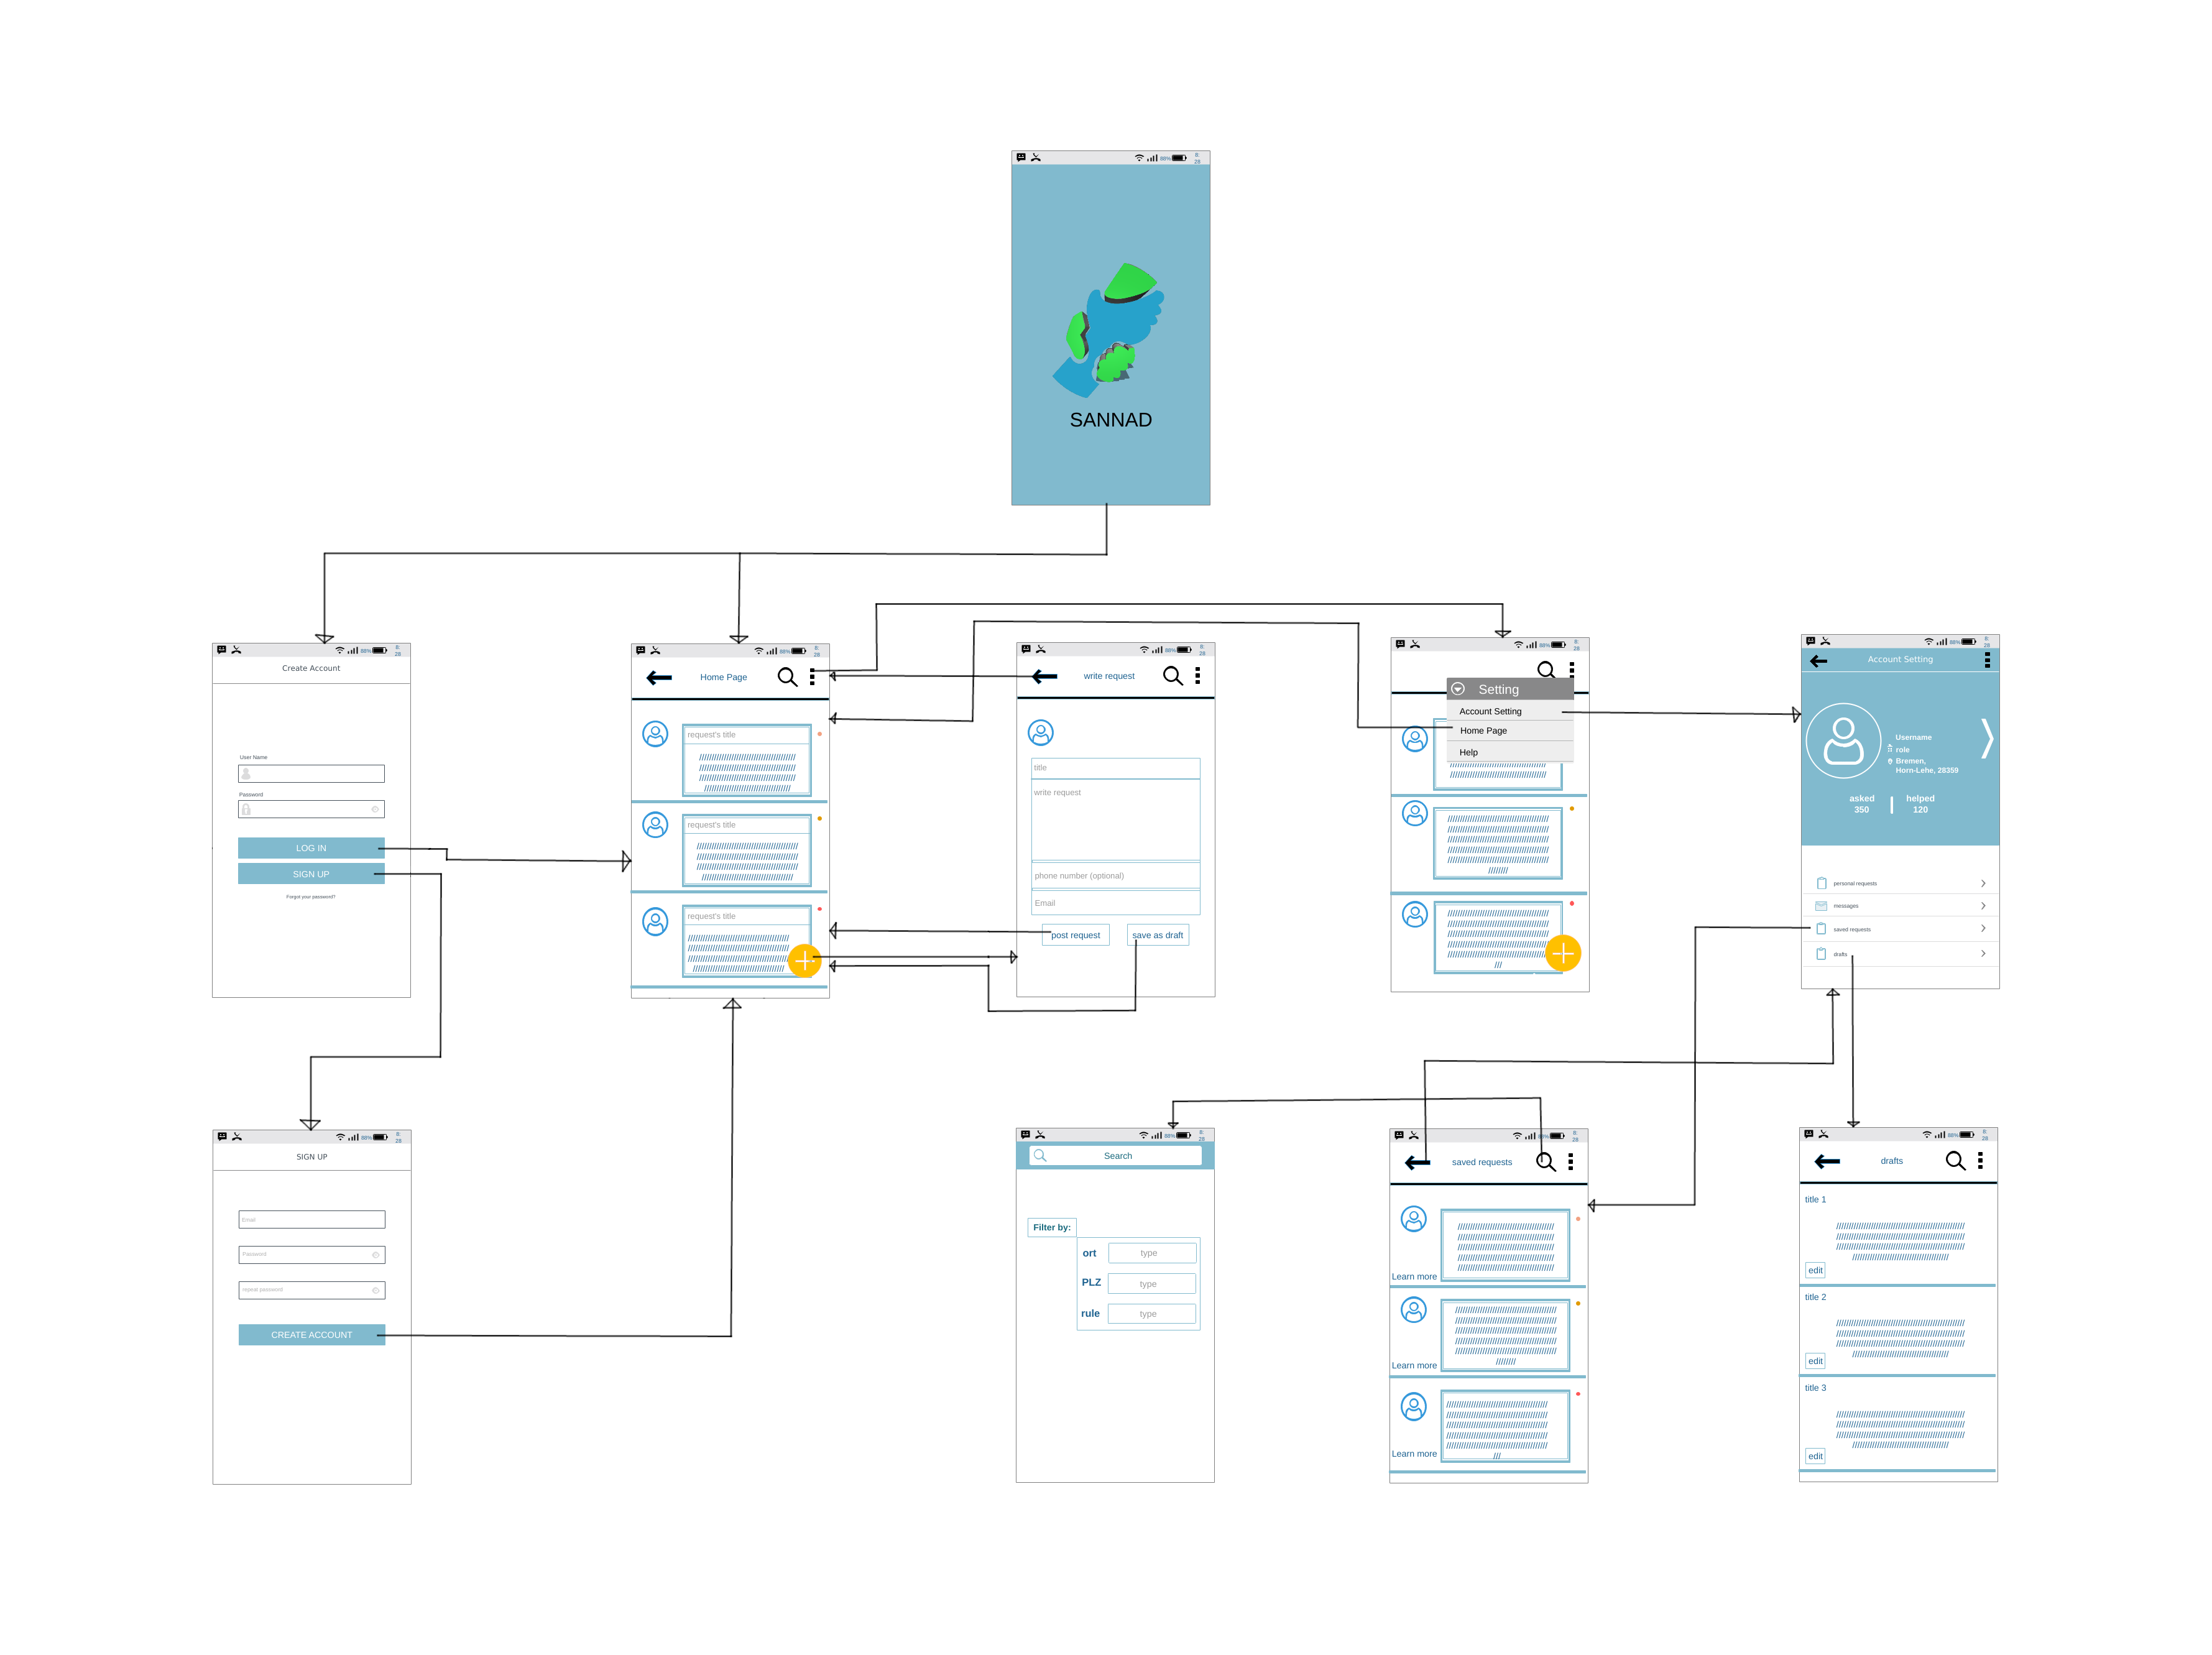
\includegraphics[width = \linewidth ]{prototyp.png}
\end{figure}

Beim starten der App wird das Logo angezeigt und kurz später wird man entweder vom Login-screen gegreetet, oder wenn man schon eingeloggt ist vom Home-screen. Im Login-screen kann man sich entweder mit einem existierenden Account anmelden oder einen neuen erstellen durch Druck auf den Create Account Knopf. Zur Speicherung der Daten benutzen wir eine Google Flask Datenbank.

Dann wird man nach der Anmeldung auf dem Home Screen landen wo man viele Requests von Menschen im gleichen Ort/Stadt sehen kann. Um eine Anzeige genauer zu betrachten, drückt man auf diese und sieht eine detailliertere Anzeige, mit den Daten der Person welche Hilfe benötigt. Die Anzeigen können außerdem filtriert und durchsucht werden nach Name, Ort, Art der benötigten Hilfe und ähnliches.

Durch druck auf die drei Punkte oben rechts kommt man auf die eigenen Details, wo man sowohl Foto wie auch andere persönliche Daten eingeben kann, wie z.B. Telefonnummer um Kontakt aufzunehmen.

Man kann dort außerdem seinen Account löschen wenn man dieses möchte. 

\underline{\textbf{Navigationsbaum:}}

Hier noch einmal ein detaillierter Navigationsbaum:

\begin{figure}[h!]
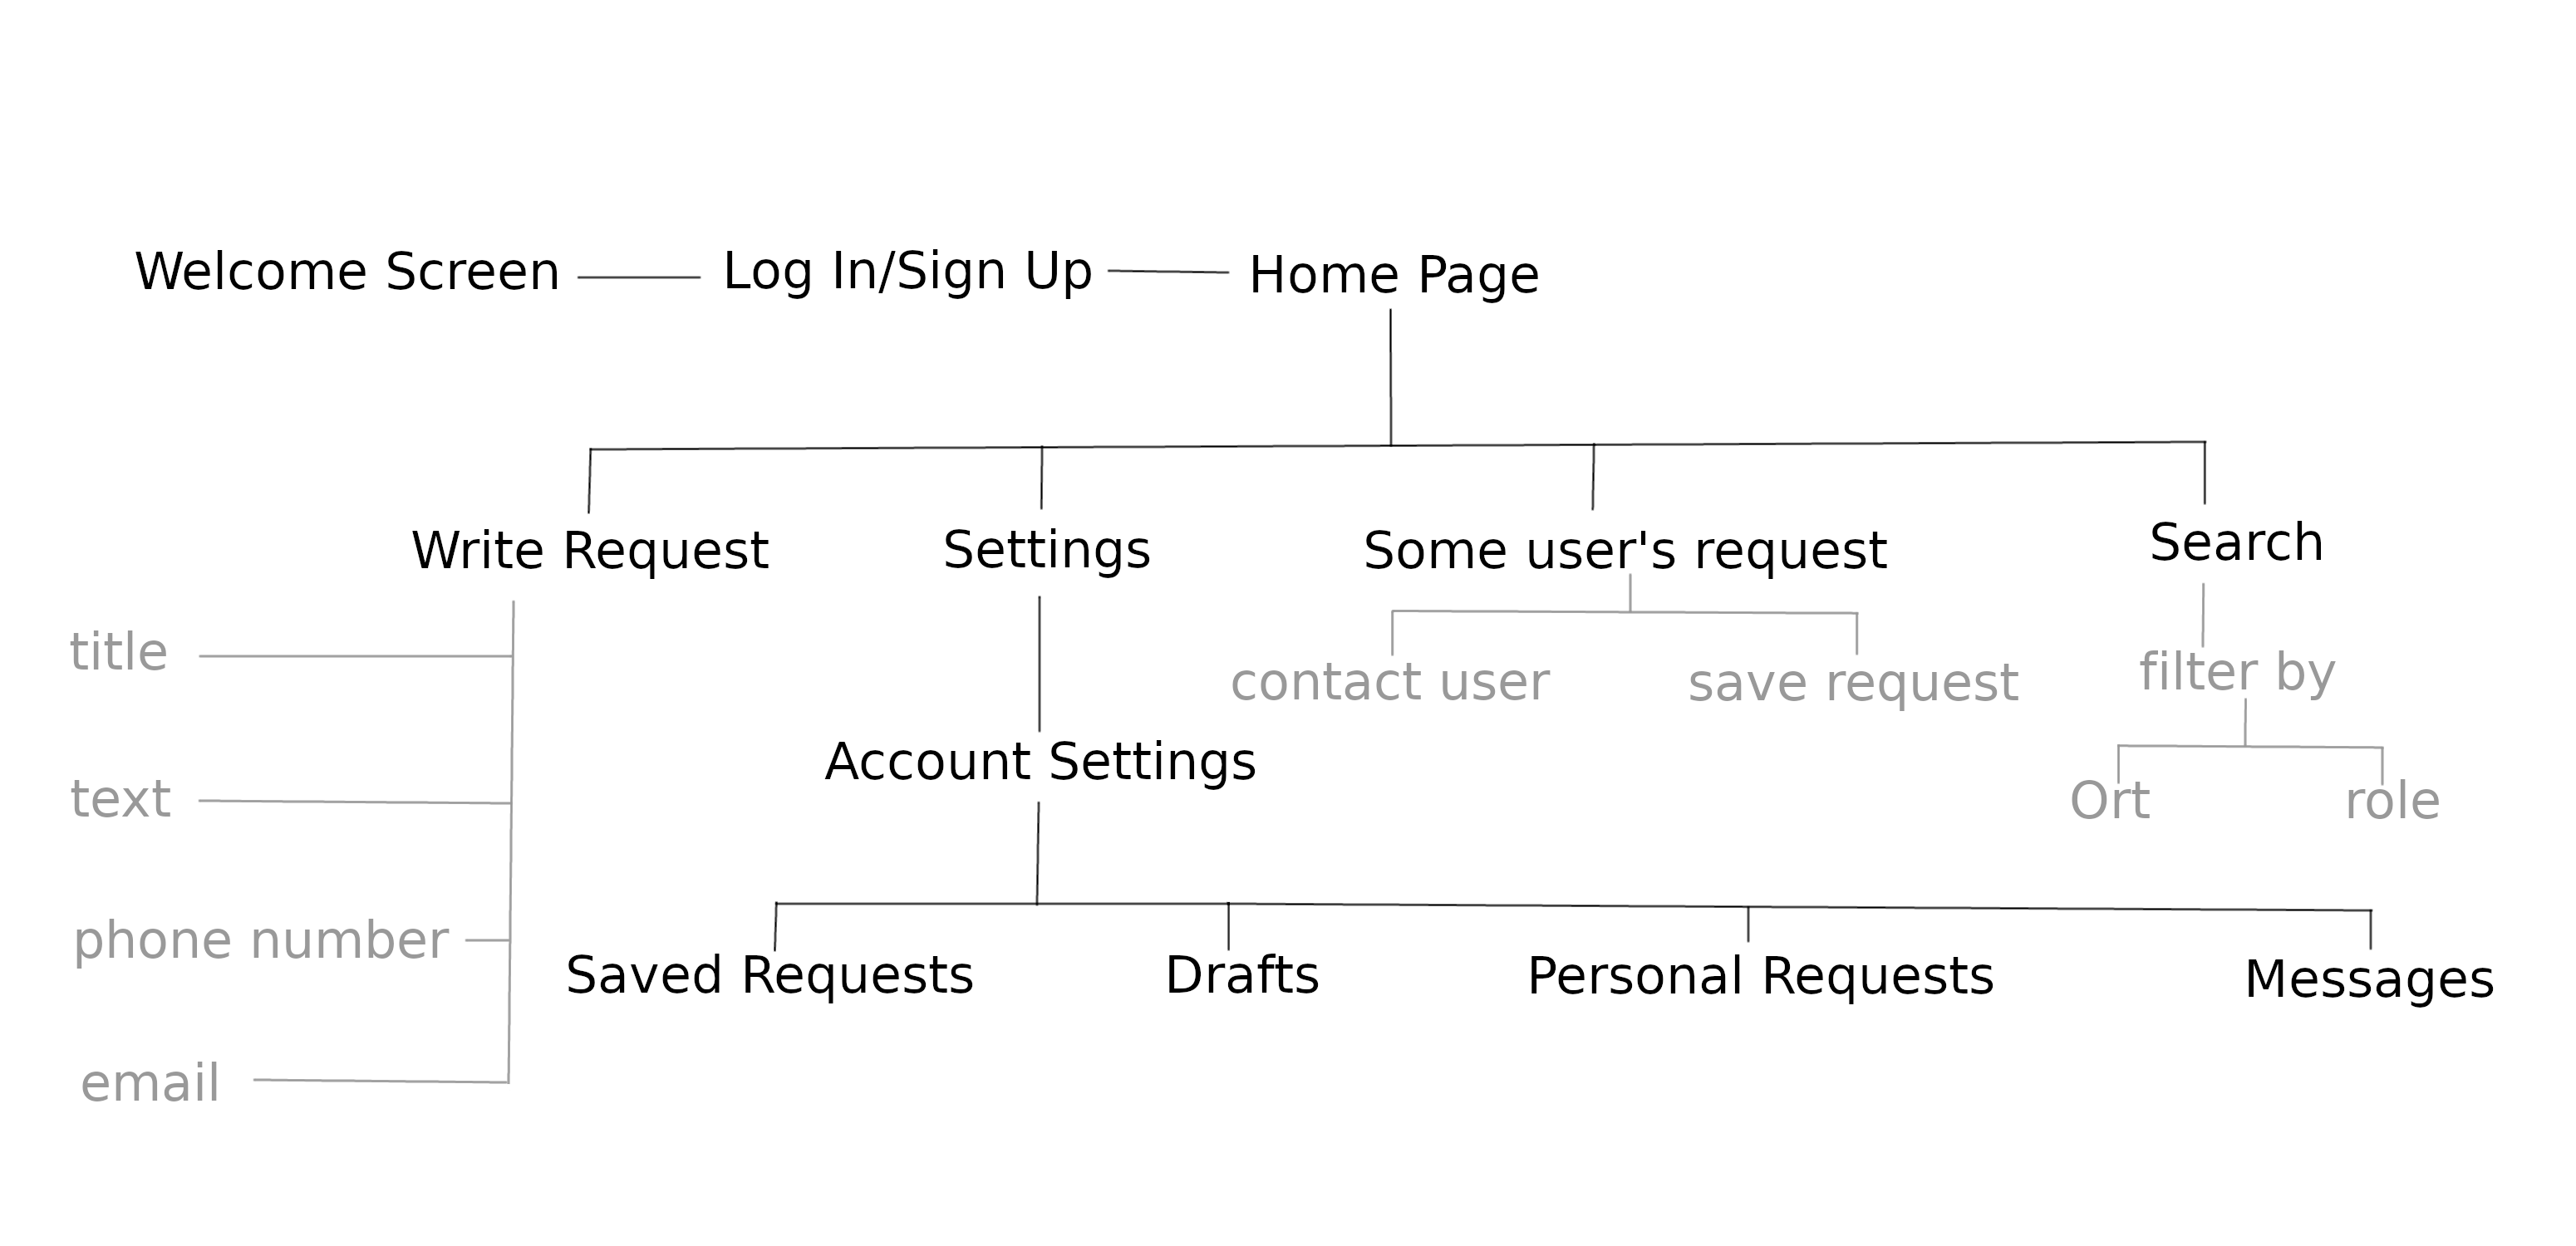
\includegraphics[width=\linewidth]{baum.png}
\end{figure}  

\end{document}